\chapter{Aufgabenstellung}
Aufgabe der Gruppe war es, zwei Firewalls zu konfigurieren. In Abb. \ref{fig:netzplan} sind diese Firewalls als fw1.firma-a.f223 und fw2.firma-a.f223 gekennzeichnet. fw1 trennt die DMZ der Firma A vom (simulierten) Internet, fw2 trennt die DMZ von Firma A vom LAN der Firma A. Dabei war gefordert, dass durch fw1 Zugriff auf die in der DMZ bereit gestellten Dienste (Webserver und Mailserver) möglich sein muss. Von außen sowie aus der DMZ soll auf das LAN hinter fw2 kein Zugriff möglich sein. Beide Firewalls sollten außerdem eine Network-Address-Translation (NAT) durchführen, bei der jeweils ein so genanntes "`Masquerading"' durchzuführen war, sodass die hinter der Firewall geschützten Rechner nach außen jeweils mit der IP-Adresse der Firewall in Erscheinung treten.

Zusätzlich zur Firewallkonfiguration war es eine weitere Aufgabe auf fw2 einen OpenVPN-Server im bridged mode für eine Client2LAN-VPN Verbindung zu konfigurieren. Diese sollte es einem simulierten Road-Warrior (in Abb. \ref{fig:netzplan} lap01.internet.f223) ermöglichen auf das Firmen-LAN und auch auf Web- und Mailserver zuzugreifen.

\begin{figure}[h!]
	\centering
		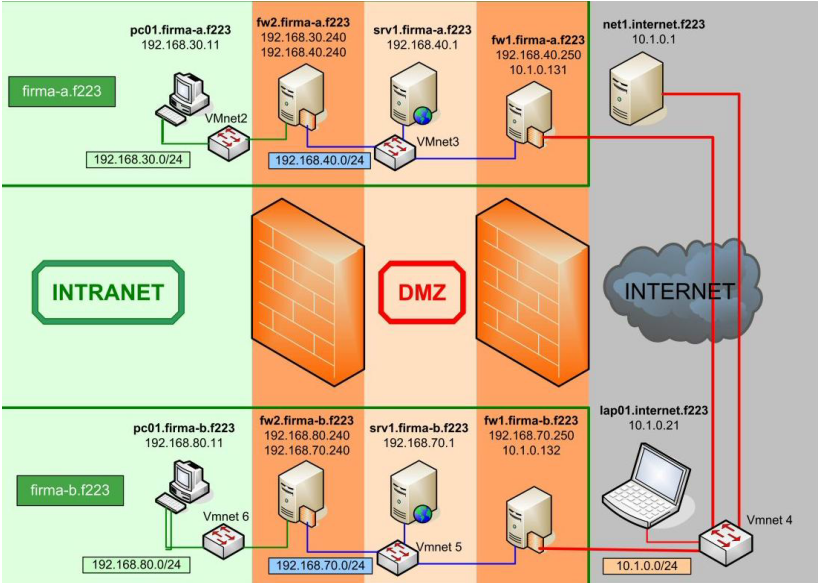
\includegraphics[width=0.7\textwidth]{figures/netzplan.PNG}
	\caption{Netzplan \cite{Neuschwander2014}}
	\label{fig:netzplan}
\end{figure}

\chapter{Konfiguration}
Auf beiden virtuellen Maschinen wurde jeweils Debian 7 ("`Wheezy"') installiert. Anschließend mussten die Netzwerkinterfaces beider Maschinen so angepasst werden, dass Sie den Vorgaben aus \ref{fig:netzplan} entsprachen. Dies wurde durch das Eintragen entsprechender Änderungen in der Datei /etc/network/interfaces erreicht.

Für die äußere Firewall ergibt sich so folgende Konfiguration (Kommentarzeilen entfernt):
\begin{lstlisting}
auto lo
iface lo inet loopback

allow-hotplug eth0
iface eth0 inet static
	address 192.168.40.250
	netmask 255.255.255.0
	network 192.168.40.0
	broadcast 192.168.40.255
	dns-nameservers 192.168.40.1
	dns-search firma-a.f223

allow-hotplug eth1
iface eth1 inet static
	address 10.1.0.131
	netmask 255.255.255.0
	network 10.1.0.0
	broadcast 10.1.0.255
\end{lstlisting}
eth0 ist in diesem Fall die Schnittstelle in die DMZ. Entsprechend ist sie im IP-Adress-Bereich 192.168.40.0/24 angesiedelt und verwendet srv1.firma-a.f223 als DNS-Server und komplettiert DNS-Anfragen mit der Domäne firma-a.f223. eth1 ist die Schnittstelle ins simulierte Internet (Adressbereich 10.1.0.0/24).

Für die innere Firewall ist die Netzwerkkonfiguration folgende:
\begin{lstlisting}
auto lo eth0 eth1
iface lo inet loopback

allow-hotplug eth0
iface eth0 inet static
	address 192.168.30.240
	netmask 255.255.255.0
	network 192.168.30.0
	broadcast 192.168.30.255
	dns-nameservers 192.168.40.1
	dns-search firma-a.f223

allow-hotplug eth1
iface eth1 inet static
	address 192.168.40.240
	netmask 255.255.255.0
	network 192.168.40.0
	broadcast 192.168.40.255
	gateway 192.168.40.250
	dns-nameservers 192.168.40.1
	dns-search firma-a.f223
\end{lstlisting}

eth0 ist hier die Schnittstelle ins geschützte Firmen-LAN im Adressbereich 192.168.30.0/24. Auch hier fungiert srv1.firma-a.f223 als DNS-Server. Als Schnittstelle in die DMZ wird hier eth1 eingesetzt, weshalb auch hier eine Adresse aus dem Bereich 192.168.40.0/24 eingesetzt wird. Wichtig ist hier außerdem, dass die äußere Firewall als Gateway gesetzt wurde, um Netzwerkverkehr ins simulierte Internet zu erlauben. Die äußere Firewall ist das Gateway ins Internet, während die innere Firewall für die Rechner im LAN als Gateway in die DMZ eingestellt ist.
